% Chapter 2: ARMA Models
% Harvard-quality academic presentation
% Bachelor program, Bucharest University of Economic Studies

\documentclass[9pt, aspectratio=169, t]{beamer}

% Ensure content fits on slides
\setbeamersize{text margin left=8mm, text margin right=8mm}

%=============================================================================
% THEME AND STYLE CONFIGURATION
%=============================================================================
\usetheme{default}
% Using default theme for clean header/footer control

% Color Palette (matching Redispatch PDF)
\definecolor{MainBlue}{RGB}{26, 58, 110}
\definecolor{AccentBlue}{RGB}{26, 58, 110}
\definecolor{IDAred}{RGB}{205, 0, 0}
\definecolor{DarkGray}{RGB}{51, 51, 51}
\definecolor{MediumGray}{RGB}{128, 128, 128}
\definecolor{LightGray}{RGB}{248, 248, 248}
\definecolor{VeryLightGray}{RGB}{235, 235, 235}
\definecolor{KeynoteGray}{RGB}{218, 218, 218}
\definecolor{SectionGray}{RGB}{120, 120, 120}
\definecolor{FooterGray}{RGB}{100, 100, 100}
\definecolor{Crimson}{RGB}{220, 53, 69}
\definecolor{Forest}{RGB}{46, 125, 50}
\definecolor{Amber}{RGB}{181, 133, 63}
\definecolor{Orange}{RGB}{230, 126, 34}
\definecolor{Purple}{RGB}{142, 68, 173}

% Gradient background (exact Keynote 315° gradient: white to RGB 218,218,218)
\setbeamertemplate{background}{%
    \begin{tikzpicture}[remember picture, overlay]
        \shade[shading=axis, shading angle=315,
        top color=white, bottom color=KeynoteGray]
        (current page.south west) rectangle (current page.north east);
    \end{tikzpicture}%
}
% Fallback solid color for compatibility
\setbeamercolor{background canvas}{bg=}

\setbeamercolor{palette primary}{bg=MainBlue, fg=white}
\setbeamercolor{palette secondary}{bg=MainBlue!85, fg=white}
\setbeamercolor{palette tertiary}{bg=MainBlue!70, fg=white}
\setbeamercolor{structure}{fg=MainBlue}
\setbeamercolor{title}{fg=IDAred}
\setbeamercolor{frametitle}{fg=IDAred, bg=}
\setbeamercolor{block title}{bg=MainBlue, fg=white}
\setbeamercolor{block body}{bg=VeryLightGray, fg=DarkGray}
\setbeamercolor{block title alerted}{bg=Crimson, fg=white}
\setbeamercolor{block body alerted}{bg=Crimson!8, fg=DarkGray}
\setbeamercolor{block title example}{bg=Forest, fg=white}
\setbeamercolor{block body example}{bg=Forest!8, fg=DarkGray}
\setbeamercolor{item}{fg=MainBlue}

% Footer colors (override Madrid theme blue)
\setbeamercolor{author in head/foot}{fg=FooterGray, bg=}
\setbeamercolor{title in head/foot}{fg=FooterGray, bg=}
\setbeamercolor{date in head/foot}{fg=FooterGray, bg=}
\setbeamercolor{section in head/foot}{fg=FooterGray, bg=}
\setbeamercolor{subsection in head/foot}{fg=FooterGray, bg=}

% Bullet styles (apply everywhere including blocks)
\setbeamertemplate{itemize item}{\color{MainBlue}$\boxdot$}
\setbeamertemplate{itemize subitem}{\color{MainBlue}$\blacktriangleright$}
\setbeamertemplate{itemize subsubitem}{\color{MainBlue}\tiny$\bullet$}
\setbeamertemplate{itemize/enumerate body begin}{\normalsize}
\setbeamertemplate{itemize/enumerate subbody begin}{\normalsize}

% Item spacing
\setlength{\leftmargini}{1.5em}
\setlength{\leftmarginii}{1.5em}

\setbeamertemplate{navigation symbols}{}

% TOC with bullets
\setbeamertemplate{section in toc}{\color{MainBlue}$\boxdot$\hspace{0.5em}\inserttocsection}

%=============================================================================
% CUSTOM HEADLINE
%=============================================================================
\setbeamertemplate{headline}{%
    \vskip10pt%
    \hbox to \paperwidth{%
        \hskip0.5cm%
        {\small\color{FooterGray}\renewcommand{\hyperlink}[2]{##2}\insertsectionhead}%
        \hfill%
        \textcolor{FooterGray}{\small\insertframenumber}%
        \hskip0.5cm%
    }%
    \vskip4pt%
    {\color{FooterGray}\hrule height 0.4pt}%
}

%=============================================================================
% CUSTOM FOOTER
%=============================================================================
\usepackage{fontawesome5}

\setbeamertemplate{footline}{%
    {\color{FooterGray}\hrule height 0.4pt}%
    \vskip4pt%
    \hbox to \paperwidth{%
        \hskip0.5cm%
        \textcolor{FooterGray}{\small Time Series Analysis and Forecasting}%
        \hfill%
        \raisebox{-0.1em}{%
            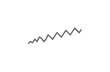
\begin{tikzpicture}[x=0.08em, y=0.08em, line width=0.4pt]
                \draw[FooterGray] (0,3) -- (1,4) -- (2,3.5) -- (3,5) -- (4,4) -- (5,6) -- (6,5.5) -- (7,4) -- (8,5) -- (9,7) -- (10,6) -- (11,5) -- (12,6.5) -- (13,8) -- (14,7) -- (15,6) -- (16,7.5) -- (17,9) -- (18,8) -- (19,7) -- (20,8.5) -- (21,10) -- (22,9) -- (23,8) -- (24,9.5);
            \end{tikzpicture}%
        }%
        \hskip0.5cm%
    }%
    \vskip6pt%
}

%=============================================================================
% PACKAGES
%=============================================================================
\usepackage[utf8]{inputenc}
\usepackage[T1]{fontenc}
\usepackage{amsmath, amssymb, amsthm}
\usepackage{mathtools}
\usepackage{bm}
\usepackage{tikz}
\usetikzlibrary{arrows.meta, positioning, shapes, calc, decorations.pathreplacing, shadings}
\usepackage{booktabs}
\usepackage{multirow}
\usepackage{array}
\usepackage{graphicx}
\usepackage{hyperref}
\usepackage{colortbl}
\hypersetup{colorlinks=true, linkcolor=MainBlue, urlcolor=MainBlue}
\graphicspath{{../logos/}{../charts/}}

%=============================================================================
% QUANTLET COMMAND
%=============================================================================
\newcommand{\quantlet}[2]{%
    \begin{tikzpicture}[remember picture, overlay]
        \node[anchor=south east, inner sep=0pt] at ([xshift=-0.5cm, yshift=0.75cm]current page.south east) {%
            \href{#2}{%
                \raisebox{-0.1em}{\includegraphics[height=0.8em]{ql_logo.png}}%
                \textcolor{MainBlue}{\scriptsize\ #1}%
            }%
        };
    \end{tikzpicture}%
}

%=============================================================================
% CUSTOM TITLE PAGE
%=============================================================================
\defbeamertemplate*{title page}{hybrid}[1][]
{
    \vspace{0.2cm}
    % Logos row - top header (with clickable links)
    \begin{center}
        \href{https://www.ase.ro}{\includegraphics[height=0.9cm]{ase_logo.png}}\hspace{0.15cm}%
        \href{https://theida.net}{\includegraphics[height=0.9cm]{ida_logo.png}}\hspace{0.15cm}%
        \href{https://blockchain-research-center.com}{\includegraphics[height=0.9cm]{brc_logo.png}}\hspace{0.15cm}%
        \href{https://www.ai4efin.ase.ro}{\includegraphics[height=0.9cm]{ai4efin_logo.png}}\hspace{0.15cm}%
        \href{https://ipe.ro/new}{\includegraphics[height=0.9cm]{acad_logo.png}}\hspace{0.15cm}%
        \href{https://www.digital-finance-msca.com}{\includegraphics[height=0.9cm]{msca_logo.png}}%
    \end{center}

    \vspace{0.6cm}

    % Main title with Q logos on sides (with clickable links)
    \begin{center}
        \begin{minipage}{0.10\textwidth}
            \centering
            \href{https://quantlet.com}{\includegraphics[height=1.0cm]{ql_logo.png}}
        \end{minipage}%
        \begin{minipage}{0.76\textwidth}
            \centering
            {\LARGE\bfseries\usebeamercolor[fg]{title}\inserttitle}

            \vspace{0.3cm}

            {\usebeamerfont{subtitle}\usebeamercolor[fg]{title}\insertsubtitle}
        \end{minipage}%
        \begin{minipage}{0.10\textwidth}
            \centering
            \href{https://quantinar.com}{\includegraphics[height=1.0cm]{qr_logo.png}}
        \end{minipage}
    \end{center}

    \vspace{0.6cm}

    % Authors (left aligned)
    \hspace{0.5cm}{\usebeamerfont{author}\insertauthor}

    \vspace{0.3cm}

    % Institute/Affiliations (left aligned)
    \hspace{0.5cm}\begin{minipage}[t]{0.9\textwidth}
        \raggedright\small\insertinstitute
    \end{minipage}
}

%=============================================================================
% THEOREM ENVIRONMENTS
%=============================================================================
\theoremstyle{definition}
\setbeamertemplate{theorems}[numbered]
\newtheorem{defn}{Definition}
\newtheorem{thm}{Theorem}
\newtheorem{prop}{Proposition}
\newtheorem{rmk}{Remark}

%=============================================================================
% CUSTOM COMMANDS
%=============================================================================
\newcommand{\E}{\mathbb{E}}
\newcommand{\Var}{\text{Var}}
\newcommand{\Cov}{\text{Cov}}
\newcommand{\Corr}{\text{Corr}}
\newcommand{\R}{\mathbb{R}}
\newcommand{\N}{\mathbb{N}}
\newcommand{\Z}{\mathbb{Z}}
\newcommand{\B}{\mathbf{B}}
\newcommand{\imark}{\textcolor{MainBlue}{\textbullet}}
\newcommand{\RMSE}{\text{RMSE}}
\newcommand{\MAE}{\text{MAE}}
\newcommand{\MAPE}{\text{MAPE}}

%=============================================================================
% TITLE INFORMATION
%=============================================================================
\title[Time Series Analysis]{Time Series Analysis and Forecasting}
\subtitle{Chapter 2: ARMA Models}
\author[D.T. Pele]{Daniel Traian PELE}
\institute{Bucharest University of Economic Studies\\
IDA Institute Digital Assets\\
Blockchain Research Center\\
AI4EFin Artificial Intelligence for Energy Finance\\
Romanian Academy, Institute for Economic Forecasting\\
MSCA Digital Finance}
\date{}

\begin{document}

% Title page (no header/footer)
{
\setbeamertemplate{headline}{}
\setbeamertemplate{footline}{}
\begin{frame}
    \titlepage
\end{frame}
}

%=============================================================================
% TABLE OF CONTENTS
%=============================================================================
\begin{frame}{Outline}
    \tableofcontents
\end{frame}

%=============================================================================
% MOTIVATION
%=============================================================================
\section{Motivation}

\begin{frame}{Motivating Example: Stationary Processes}
    \vspace{-0.3cm}
    \begin{center}
        \includegraphics[width=0.92\textwidth, height=0.62\textheight, keepaspectratio]{ch2_motivation_stationary.pdf}
    \end{center}
    \vspace{-0.2cm}
    {\footnotesize
    \begin{itemize}
        \item \textbf{AR processes}: Current value depends on past values --- mean-reverting behavior
        \item \textbf{MA processes}: Current value depends on past shocks --- short memory
        \item \textbf{ARMA}: Combines both mechanisms for flexible modeling
    \end{itemize}
    }
    \quantlet{TSA\_ch2\_motivation}{https://github.com/QuantLet/TSA/tree/main/TSA_ch2/TSA_ch2_motivation}
\end{frame}

\begin{frame}{Model Identification via ACF Patterns}
    \vspace{-0.3cm}
    \begin{center}
        \includegraphics[width=0.95\textwidth, height=0.58\textheight, keepaspectratio]{ch2_motivation_acf.pdf}
    \end{center}
    \vspace{-0.2cm}
    {\footnotesize
    \begin{exampleblock}{The ACF Reveals Model Structure}
        \begin{itemize}
            \item Different ARMA models produce distinct ACF patterns
            \item We can identify the model by examining the data!
        \end{itemize}
    \end{exampleblock}
    }
    \quantlet{TSA\_ch2\_motivation}{https://github.com/QuantLet/TSA/tree/main/TSA_ch2/TSA_ch2_motivation}
\end{frame}

%=============================================================================
% SECTION 1: INTRODUCTION AND LAG OPERATOR
%=============================================================================
\section{Introduction and Lag Operator}

\begin{frame}{Recap: Stationarity}
    \textbf{From Chapter 1:} A process $\{X_t\}$ is \textbf{weakly stationary} if:
    \begin{enumerate}
        \item $\E[X_t] = \mu$ (constant mean)
        \item $\Var(X_t) = \sigma^2 < \infty$ (constant, finite variance)
        \item $\Cov(X_t, X_{t+h}) = \gamma(h)$ (covariance depends only on lag $h$)
    \end{enumerate}

    \vspace{0.15cm}
    \textbf{Why stationarity matters for ARMA:}
    \begin{itemize}
        \item ARMA models assume the underlying process is stationary
        \item Non-stationary data must be differenced first (ARIMA)
        \item Stationarity ensures stable model parameters
    \end{itemize}

    \vspace{0.15cm}
    \textbf{Today:} We build models for stationary time series using past values and past errors.
\end{frame}

\begin{frame}{The Lag Operator (Backshift Operator)}
    \begin{defn}[Lag Operator]
        The \textbf{lag operator} $L$ (or backshift operator $B$) shifts a time series back by one period:
        $$L X_t = X_{t-1}$$
    \end{defn}

    \textbf{Properties:}
    \begin{itemize}
        \item $L^k X_t = X_{t-k}$ (shift back $k$ periods)
        \item $L^0 X_t = X_t$ (identity)
        \item $(1-L)X_t = X_t - X_{t-1} = \Delta X_t$ (first difference)
        \item $(1-L)^d X_t = \Delta^d X_t$ ($d$-th difference)
    \end{itemize}

    \vspace{0.15cm}
    \textbf{Lag Polynomials:}
    $$\phi(L) = 1 - \phi_1 L - \phi_2 L^2 - \cdots - \phi_p L^p$$
    $$\theta(L) = 1 + \theta_1 L + \theta_2 L^2 + \cdots + \theta_q L^q$$
    \quantlet{TSA\_ch2\_lag\_operator}{https://github.com/QuantLet/TSA/tree/main/TSA_ch2/TSA_ch2_lag_operator}
\end{frame}

\begin{frame}{Lag Operator: Visual Illustration}
    \begin{center}
        \includegraphics[width=0.95\textwidth, height=0.55\textheight, keepaspectratio]{lag_operator.pdf}
    \end{center}
    \vspace{-0.2cm}
    {\footnotesize
    \begin{exampleblock}{Key Insight}
        \begin{itemize}
            \item $L$ shifts observations back: $LX_t = X_{t-1}$; simplifies ARMA expressions
        \end{itemize}
    \end{exampleblock}
    }
    \quantlet{TSA\_ch2\_lag\_operator}{https://github.com/QuantLet/TSA/tree/main/TSA_ch2/TSA_ch2_lag_operator}
\end{frame}

\begin{frame}{White Noise Process}
    \begin{defn}[White Noise]
        A process $\{\varepsilon_t\}$ is \textbf{white noise}, denoted $\varepsilon_t \sim WN(0, \sigma^2)$, if:
        \begin{enumerate}
            \item $\E[\varepsilon_t] = 0$ for all $t$
            \item $\Var(\varepsilon_t) = \sigma^2$ for all $t$
            \item $\Cov(\varepsilon_t, \varepsilon_s) = 0$ for all $t \neq s$
        \end{enumerate}
    \end{defn}

    \vspace{0.15cm}
    \textbf{Properties:}
    \begin{itemize}
        \item White noise is the ``building block'' of ARMA models
        \item ACF: $\rho(0) = 1$, $\rho(h) = 0$ for $h \neq 0$
        \item PACF: same pattern
        \item \textbf{Gaussian white noise:} additionally $\varepsilon_t \sim N(0, \sigma^2)$
    \end{itemize}

    \vspace{0.15cm}
    \textbf{Note:} White noise is \textit{not} predictable --- it's pure randomness.
\end{frame}

\begin{frame}{White Noise: Visual Illustration}
    \begin{center}
        \includegraphics[width=0.95\textwidth, height=0.52\textheight, keepaspectratio]{ch2_white_noise.pdf}
    \end{center}
    \vspace{-0.2cm}
    {\footnotesize
    \begin{block}{Key Characteristics}
        \begin{itemize}
            \item \textbf{Left}: Series fluctuates randomly around mean zero with no patterns
            \item \textbf{Right}: ACF shows only spike at lag 0; all others within confidence bounds
        \end{itemize}
    \end{block}
    }
    \quantlet{TSA\_ch2\_white\_noise}{https://github.com/QuantLet/TSA/tree/main/TSA_ch2/TSA_ch2_white_noise}
\end{frame}

%=============================================================================
% SECTION 2: AR MODELS
%=============================================================================
\section{Autoregressive (AR) Models}

\begin{frame}{AR(1) Model: Definition}
    \begin{defn}[AR(1) Process]
        An \textbf{autoregressive process of order 1} is:
        $$X_t = c + \phi X_{t-1} + \varepsilon_t$$
        where $\varepsilon_t \sim WN(0, \sigma^2)$ and $|\phi| < 1$ for stationarity.
    \end{defn}

    \vspace{0.15cm}
    \textbf{Interpretation:}
    \begin{itemize}
        \item $c$: constant (intercept)
        \item $\phi$: autoregressive coefficient --- measures persistence
        \item $\varepsilon_t$: innovation (unpredictable shock)
    \end{itemize}

    \vspace{0.15cm}
    \textbf{Using lag operator:}
    $$(1 - \phi L)X_t = c + \varepsilon_t$$
    $$\phi(L) X_t = c + \varepsilon_t \quad \text{where } \phi(L) = 1 - \phi L$$
\end{frame}

\begin{frame}{AR(1): Visual Illustration}
    \begin{center}
        \includegraphics[width=0.95\textwidth, height=0.50\textheight, keepaspectratio]{ch2_def_ar1.pdf}
    \end{center}
    \vspace{-0.3cm}
    {\footnotesize
    \begin{itemize}
        \item \textbf{Positive $\phi$}: Persistent, smooth fluctuations; gradual mean reversion
        \item \textbf{Negative $\phi$}: Oscillating behavior; rapid sign changes
        \item Higher $|\phi|$ $\Rightarrow$ slower mean reversion, more persistence
    \end{itemize}
    }
    \quantlet{TSA\_ch2\_ar1\_simulation}{https://github.com/QuantLet/TSA/tree/main/TSA_ch2/TSA_ch2_ar1_simulation}
\end{frame}

\begin{frame}{AR(1) Stationarity Condition}
    \textbf{For AR(1) to be stationary:} $|\phi| < 1$

    \vspace{0.15cm}
    \textbf{Intuition:}
    \begin{itemize}
        \item If $|\phi| < 1$: shocks decay over time $\rightarrow$ stationary
        \item If $|\phi| = 1$: random walk $\rightarrow$ non-stationary (unit root)
        \item If $|\phi| > 1$: explosive process $\rightarrow$ non-stationary
    \end{itemize}

    \vspace{0.15cm}
    \textbf{Characteristic equation:}
    $$\phi(z) = 1 - \phi z = 0 \implies z = \frac{1}{\phi}$$

    Stationarity requires the root $z = 1/\phi$ to lie \textbf{outside the unit circle}, i.e., $|z| > 1$, which means $|\phi| < 1$.
\end{frame}

\begin{frame}{AR(1) Properties}
    For a stationary AR(1) with $|\phi| < 1$:

    \vspace{0.15cm}
    \textbf{Mean:}
    $$\mu = \E[X_t] = \frac{c}{1-\phi}$$

    \textbf{Variance:}
    $$\gamma(0) = \Var(X_t) = \frac{\sigma^2}{1-\phi^2}$$

    \textbf{Autocovariance:}
    $$\gamma(h) = \phi^h \gamma(0) = \frac{\phi^h \sigma^2}{1-\phi^2}$$

    \textbf{Autocorrelation (ACF):}
    $$\rho(h) = \phi^h$$

    \textbf{Key insight:} ACF decays exponentially at rate $\phi$
    \quantlet{TSA\_ch2\_ar1}{https://github.com/QuantLet/TSA/tree/main/TSA_ch2/TSA_ch2_ar1}
\end{frame}

\begin{frame}{Proof: AR(1) Mean}
    \textbf{Claim:} For AR(1): $X_t = c + \phi X_{t-1} + \varepsilon_t$, the mean is $\mu = \frac{c}{1-\phi}$

    \vspace{0.2cm}
    \textbf{Proof:} Take expectations of both sides:
    $$\E[X_t] = \E[c + \phi X_{t-1} + \varepsilon_t] = c + \phi \E[X_{t-1}] + \E[\varepsilon_t]$$

    By stationarity, $\E[X_t] = \E[X_{t-1}] = \mu$, and $\E[\varepsilon_t] = 0$:
    $$\mu = c + \phi \mu$$

    Solving for $\mu$:
    $$\mu - \phi\mu = c \implies \mu(1-\phi) = c \implies \boxed{\mu = \frac{c}{1-\phi}}$$

    \vspace{0.1cm}
    \begin{alertblock}{Requirement}
        This requires $\phi \neq 1$. If $\phi = 1$ (unit root), the mean is undefined.
    \end{alertblock}
\end{frame}

\begin{frame}{Proof: AR(1) Variance}
    \textbf{Claim:} $\Var(X_t) = \frac{\sigma^2}{1-\phi^2}$

    \vspace{0.15cm}
    \textbf{Proof:} Without loss of generality, assume $c=0$ (centered process):
    $$\Var(X_t) = \Var(\phi X_{t-1} + \varepsilon_t) = \phi^2 \Var(X_{t-1}) + \Var(\varepsilon_t) + 2\phi\Cov(X_{t-1}, \varepsilon_t)$$

    Since $\varepsilon_t$ is independent of $X_{t-1}$, $\Cov(X_{t-1}, \varepsilon_t) = 0$:
    $$\gamma(0) = \phi^2 \gamma(0) + \sigma^2$$

    By stationarity, $\Var(X_t) = \Var(X_{t-1}) = \gamma(0)$:
    $$\gamma(0) - \phi^2\gamma(0) = \sigma^2 \implies \gamma(0)(1-\phi^2) = \sigma^2 \implies \boxed{\gamma(0) = \frac{\sigma^2}{1-\phi^2}}$$

    \begin{exampleblock}{Note}
        \begin{itemize}
            \item Requires $|\phi| < 1$ for positive variance
            \item As $|\phi| \to 1$, variance $\to \infty$
        \end{itemize}
    \end{exampleblock}
\end{frame}

\begin{frame}{Proof: AR(1) Autocorrelation Function}
    \textbf{Claim:} $\rho(h) = \phi^h$ for $h \geq 0$

    \vspace{0.15cm}
    \textbf{Proof:} First, find autocovariance $\gamma(h) = \Cov(X_t, X_{t-h})$.

    Multiply $X_t = \phi X_{t-1} + \varepsilon_t$ by $X_{t-h}$ and take expectations:
    $$\E[X_t X_{t-h}] = \phi \E[X_{t-1} X_{t-h}] + \E[\varepsilon_t X_{t-h}]$$

    For $h \geq 1$: $\E[\varepsilon_t X_{t-h}] = 0$ (future shock uncorrelated with past values)
    $$\gamma(h) = \phi \gamma(h-1)$$

    This is a recursive relation! Starting from $\gamma(0)$:
    $$\gamma(1) = \phi\gamma(0), \quad \gamma(2) = \phi\gamma(1) = \phi^2\gamma(0), \quad \ldots \quad \boxed{\gamma(h) = \phi^h\gamma(0)}$$

    The ACF is:
    $$\rho(h) = \frac{\gamma(h)}{\gamma(0)} = \frac{\phi^h\gamma(0)}{\gamma(0)} = \boxed{\phi^h}$$
\end{frame}

\begin{frame}{AR(1) Variance as Function of $\phi$}
    \begin{center}
        \includegraphics[width=0.95\textwidth, height=0.55\textheight, keepaspectratio]{ar1_variance.pdf}
    \end{center}
    \vspace{-0.2cm}
    {\footnotesize
    \begin{alertblock}{Critical Insight}
        \begin{itemize}
            \item As $|\phi| \to 1$, variance $\sigma^2/(1-\phi^2) \to \infty$
            \item Unit root processes ($\phi = 1$) are non-stationary: unbounded variance
        \end{itemize}
    \end{alertblock}
    }
    \quantlet{TSA\_ch2\_ar1}{https://github.com/QuantLet/TSA/tree/main/TSA_ch2/TSA_ch2_ar1}
\end{frame}

\begin{frame}{AR(1) Simulations: Effect of $\phi$}
    \vspace{-0.3cm}
    \begin{center}
        \includegraphics[width=0.82\textwidth, height=0.58\textheight, keepaspectratio]{ch2_ar1_simulations.pdf}
    \end{center}
    \vspace{-0.2cm}
    {\footnotesize
    \begin{itemize}
        \item Different $\phi$ values produce distinct behavior: higher $|\phi|$ means more persistence
        \item Positive $\phi$ creates smooth, trending patterns; negative $\phi$ creates oscillations
        \item As $|\phi| \to 1$, the process becomes more persistent and approaches non-stationarity
    \end{itemize}
    }
    \quantlet{TSA\_ch2\_ar1\_simulation}{https://github.com/QuantLet/TSA/tree/main/TSA_ch2/TSA_ch2_ar1_simulation}
\end{frame}

\begin{frame}{AR(1) Theoretical ACF}
    \vspace{-0.2cm}
    \begin{center}
        \includegraphics[width=0.85\textwidth, height=0.50\textheight, keepaspectratio]{ar1_theoretical_acf.pdf}
    \end{center}
    \vspace{-0.2cm}
    {\footnotesize
    \begin{exampleblock}{ACF Pattern}
        \begin{itemize}
            \item For AR(1): $\rho(h) = \phi^h$
            \item Positive $\phi$: smooth decay; negative $\phi$: alternating decay
        \end{itemize}
    \end{exampleblock}
    }
    \quantlet{TSA\_ch2\_ar1}{https://github.com/QuantLet/TSA/tree/main/TSA_ch2/TSA_ch2_ar1}
\end{frame}

\begin{frame}{AR(1) ACF and PACF: Theory vs Sample}
    \vspace{-0.3cm}
    \begin{center}
        \includegraphics[width=0.82\textwidth, height=0.58\textheight, keepaspectratio]{ch2_ar1_acf_pacf.pdf}
    \end{center}
    \vspace{-0.2cm}
    {\footnotesize
    \begin{itemize}
        \item \textbf{ACF}: Exponential decay at rate $\phi$ -- theoretical formula: $\rho(h) = \phi^h$
        \item \textbf{PACF}: Single spike at lag 1, then cuts off -- this identifies AR(1)
        \item Sample estimates (bars) fluctuate around theoretical values; use confidence bands
    \end{itemize}
    }
    \quantlet{TSA\_ch2\_acf\_pacf\_patterns}{https://github.com/QuantLet/TSA/tree/main/TSA_ch2/TSA_ch2_acf_pacf_patterns}
\end{frame}

\begin{frame}{AR(1) ACF and PACF Patterns}
    \textbf{ACF of AR(1):}
    \begin{itemize}
        \item Decays exponentially: $\rho(h) = \phi^h$
        \item If $\phi > 0$: all positive, gradual decay
        \item If $\phi < 0$: alternating signs, decay in magnitude
    \end{itemize}

    \vspace{0.15cm}
    \textbf{PACF of AR(1):}
    \begin{itemize}
        \item \textbf{Cuts off after lag 1}
        \item $\pi_1 = \phi$, $\pi_k = 0$ for $k > 1$
    \end{itemize}

    \vspace{0.15cm}
    \begin{center}
    \begin{tabular}{lcc}
        \toprule
        & \textbf{ACF} & \textbf{PACF} \\
        \midrule
        AR(1) & Exponential decay & Cuts off at lag 1 \\
        \bottomrule
    \end{tabular}
    \end{center}

    \vspace{0.15cm}
    \textbf{This is the key identification pattern for AR(1)!}
\end{frame}

\begin{frame}{AR(p) Model: General Form}
    \begin{defn}[AR(p) Process]
        An \textbf{autoregressive process of order p} is:
        $$X_t = c + \phi_1 X_{t-1} + \phi_2 X_{t-2} + \cdots + \phi_p X_{t-p} + \varepsilon_t$$
    \end{defn}

    \textbf{Using lag operator:}
    $$\phi(L) X_t = c + \varepsilon_t$$
    where $\phi(L) = 1 - \phi_1 L - \phi_2 L^2 - \cdots - \phi_p L^p$

    \vspace{0.15cm}
    \textbf{Stationarity condition:}
    \begin{itemize}
        \item All roots of $\phi(z) = 0$ must lie \textbf{outside} the unit circle
        \item Equivalently: all roots have modulus $> 1$
    \end{itemize}

    \vspace{0.15cm}
    \textbf{PACF pattern:}
    \begin{itemize}
        \item PACF cuts off after lag $p$
        \item ACF decays (exponentially or with damped oscillations)
    \end{itemize}
\end{frame}

\begin{frame}{AR(p): Visual Illustration}
    \begin{center}
        \includegraphics[width=0.95\textwidth, height=0.50\textheight, keepaspectratio]{ch2_def_arp.pdf}
    \end{center}
    \vspace{-0.2cm}
    {\footnotesize
    \begin{itemize}
        \item \textbf{AR(2) with real roots}: Mixture of two exponential decays in ACF
        \item \textbf{AR(2) with complex roots}: Pseudo-cyclic behavior
            \begin{itemize}
                \item Damped sinusoidal ACF pattern
                \item Period related to argument of complex roots
            \end{itemize}
        \item \textbf{Key identification}: PACF cuts off after lag $p$ (here, lag 2)
        \item Higher-order AR models can capture richer dynamics
    \end{itemize}
    }
    \quantlet{TSA\_ch2\_ar2}{https://github.com/QuantLet/TSA/tree/main/TSA_ch2/TSA_ch2_ar2}
\end{frame}

\begin{frame}{AR(2) Stationarity: Unit Circle Visualization}
    \begin{center}
        \includegraphics[width=0.95\textwidth, height=0.55\textheight, keepaspectratio]{unit_circle_stationarity.pdf}
    \end{center}
    \vspace{-0.2cm}
    {\footnotesize
    \begin{block}{Stationarity Condition}
        \begin{itemize}
            \item All roots of $\phi(z) = 1 - \phi_1 z - \phi_2 z^2 = 0$ must lie \textbf{outside} the unit circle
            \item Equivalently, all roots must have modulus $> 1$
        \end{itemize}
    \end{block}
    }
    \quantlet{TSA\_ch2\_stationarity}{https://github.com/QuantLet/TSA/tree/main/TSA_ch2/TSA_ch2_stationarity}
\end{frame}

\begin{frame}{AR(2) Stationarity Triangle}
    \vspace{-0.3cm}
    \begin{center}
        \includegraphics[width=0.82\textwidth, height=0.58\textheight, keepaspectratio]{ch2_ar2_stationarity.pdf}
    \end{center}
    \vspace{-0.2cm}
    {\footnotesize
    \begin{itemize}
        \item The triangular region defines all stationary AR(2) parameter combinations
        \item Boundaries: $\phi_1 + \phi_2 < 1$, $\phi_2 - \phi_1 < 1$, and $|\phi_2| < 1$
        \item Points outside this region lead to non-stationary or explosive processes
    \end{itemize}
    }
    \quantlet{TSA\_ch2\_stationarity}{https://github.com/QuantLet/TSA/tree/main/TSA_ch2/TSA_ch2_stationarity}
\end{frame}

\begin{frame}{Characteristic Polynomial Roots}
    \begin{center}
        \includegraphics[width=0.95\textwidth, height=0.55\textheight, keepaspectratio]{characteristic_roots.pdf}
    \end{center}
    \vspace{-0.2cm}
    {\footnotesize
    \begin{exampleblock}{Interpretation}
        \begin{itemize}
            \item Complex conjugate roots produce oscillatory ACF behavior
            \item Closer to unit circle $\Rightarrow$ more persistent oscillations; real roots $\Rightarrow$ monotonic decay
        \end{itemize}
    \end{exampleblock}
    }
    \quantlet{TSA\_ch2\_stationarity}{https://github.com/QuantLet/TSA/tree/main/TSA_ch2/TSA_ch2_stationarity}
\end{frame}

\begin{frame}{AR(2) Model}
    \begin{defn}[AR(2) Process]
        $$X_t = c + \phi_1 X_{t-1} + \phi_2 X_{t-2} + \varepsilon_t$$
    \end{defn}

    \textbf{Stationarity conditions for AR(2):}
    \begin{enumerate}
        \item $\phi_1 + \phi_2 < 1$
        \item $\phi_2 - \phi_1 < 1$
        \item $|\phi_2| < 1$
    \end{enumerate}

    \vspace{0.15cm}
    \textbf{ACF behavior depends on roots:}
    \begin{itemize}
        \item \textbf{Real roots:} mixture of two exponential decays
        \item \textbf{Complex roots:} damped sinusoidal pattern (pseudo-cycles)
    \end{itemize}

    \vspace{0.15cm}
    \textbf{PACF:} Cuts off after lag 2 ($\pi_k = 0$ for $k > 2$)
    \quantlet{TSA\_ch2\_ar2}{https://github.com/QuantLet/TSA/tree/main/TSA_ch2/TSA_ch2_ar2}
\end{frame}

\begin{frame}{Quiz: AR Stationarity}
    \begin{alertblock}{Question}
        For which value of $\phi$ is the AR(1) process $X_t = c + \phi X_{t-1} + \varepsilon_t$ stationary?
    \end{alertblock}

    \vspace{0.3cm}

    \begin{enumerate}[(A)]
        \item $\phi = 1.2$
        \item $\phi = 1.0$
        \item $\phi = -0.8$
        \item $\phi = -1.5$
    \end{enumerate}
\end{frame}

\begin{frame}{Quiz: AR Stationarity -- Answer}
    {\footnotesize
    \begin{exampleblock}{Correct Answer: (C) $\phi = -0.8$}
        \begin{itemize}
            \item AR(1) stationary iff $|\phi| < 1$; only $|-0.8| = 0.8 < 1$
        \end{itemize}
    \end{exampleblock}
    }
    \begin{center}
        \includegraphics[width=0.95\textwidth, height=0.48\textheight, keepaspectratio]{ch2_quiz_ar_stationarity.pdf}
    \end{center}
    \quantlet{TSA\_ch2\_ar1\_simulation}{https://github.com/QuantLet/TSA/tree/main/TSA_ch2/TSA_ch2_ar1_simulation}
\end{frame}

%=============================================================================
% SECTION 3: MA MODELS
%=============================================================================
\section{Moving Average (MA) Models}

\begin{frame}{MA(1) Model: Definition}
    \begin{defn}[MA(1) Process]
        A \textbf{moving average process of order 1} is:
        $$X_t = \mu + \varepsilon_t + \theta \varepsilon_{t-1}$$
        where $\varepsilon_t \sim WN(0, \sigma^2)$.
    \end{defn}

    \vspace{0.15cm}
    \textbf{Interpretation:}
    \begin{itemize}
        \item $\mu$: mean of the process
        \item $\theta$: MA coefficient --- measures impact of past shock
        \item Current value depends on current and one past shock
    \end{itemize}

    \vspace{0.15cm}
    \textbf{Using lag operator:}
    $$X_t = \mu + \theta(L)\varepsilon_t$$
    where $\theta(L) = 1 + \theta L$

    \vspace{0.15cm}
    \textbf{Key property:} MA processes are \textbf{always stationary} for any finite $\theta$
\end{frame}

\begin{frame}{MA(1): Visual Illustration}
    \begin{center}
        \includegraphics[width=0.95\textwidth, height=0.55\textheight, keepaspectratio]{ch2_def_ma1.pdf}
    \end{center}
    \vspace{-0.2cm}
    {\footnotesize
    \begin{itemize}
        \item \textbf{Left panel}: MA(1) series --- less persistent than AR(1), rapid mean reversion
        \item \textbf{Right panel}: ACF shows characteristic \textbf{cutoff after lag 1}
            \begin{itemize}
                \item Only $\rho(1) \neq 0$; all higher lags are zero
                \item This sharp cutoff is the key identifier for MA models
            \end{itemize}
        \item PACF decays exponentially (opposite pattern to AR)
    \end{itemize}
    }
    \quantlet{TSA\_ch2\_ma1}{https://github.com/QuantLet/TSA/tree/main/TSA_ch2/TSA_ch2_ma1}
\end{frame}

\begin{frame}{MA(1) Properties}
    For MA(1): $X_t = \mu + \varepsilon_t + \theta \varepsilon_{t-1}$

    \vspace{0.15cm}
    \textbf{Mean:}
    $$\E[X_t] = \mu$$

    \textbf{Variance:}
    $$\gamma(0) = \Var(X_t) = \sigma^2(1 + \theta^2)$$

    \textbf{Autocovariance:}
    $$\gamma(1) = \theta\sigma^2, \quad \gamma(h) = 0 \text{ for } h > 1$$

    \textbf{Autocorrelation (ACF):}
    $$\rho(1) = \frac{\theta}{1+\theta^2}, \quad \rho(h) = 0 \text{ for } h > 1$$

    \vspace{0.15cm}
    \textbf{Key insight:} ACF \textbf{cuts off} after lag 1
    \quantlet{TSA\_ch2\_ma1}{https://github.com/QuantLet/TSA/tree/main/TSA_ch2/TSA_ch2_ma1}
\end{frame}

\begin{frame}{Proof: MA(1) Variance and Autocovariance}
    \textbf{Setup:} $X_t = \varepsilon_t + \theta\varepsilon_{t-1}$ (assuming $\mu = 0$)

    \vspace{0.15cm}
    \textbf{Variance:}
    \begin{align*}
    \gamma(0) &= \Var(X_t) = \Var(\varepsilon_t + \theta\varepsilon_{t-1}) \\
    &= \Var(\varepsilon_t) + \theta^2\Var(\varepsilon_{t-1}) + 2\theta\Cov(\varepsilon_t, \varepsilon_{t-1}) \\
    &= \sigma^2 + \theta^2\sigma^2 + 0 = \boxed{\sigma^2(1+\theta^2)}
    \end{align*}

    \textbf{Autocovariance at lag 1:}
    \begin{align*}
    \gamma(1) &= \Cov(X_t, X_{t-1}) = \Cov(\varepsilon_t + \theta\varepsilon_{t-1}, \varepsilon_{t-1} + \theta\varepsilon_{t-2}) \\
    &= \Cov(\varepsilon_t, \varepsilon_{t-1}) + \theta\Cov(\varepsilon_t, \varepsilon_{t-2}) + \theta\Cov(\varepsilon_{t-1}, \varepsilon_{t-1}) + \theta^2\Cov(\varepsilon_{t-1}, \varepsilon_{t-2}) \\
    &= 0 + 0 + \theta\sigma^2 + 0 = \boxed{\theta\sigma^2}
    \end{align*}

    \textbf{Autocovariance at lag $h \geq 2$:} No overlapping $\varepsilon$ terms $\Rightarrow \gamma(h) = 0$
\end{frame}

\begin{frame}{Proof: MA(1) ACF Maximum}
    \textbf{Claim:} $|\rho(1)| \leq 0.5$ for any value of $\theta$

    \vspace{0.2cm}
    \textbf{Proof:} The ACF at lag 1 is:
    $$\rho(1) = \frac{\gamma(1)}{\gamma(0)} = \frac{\theta\sigma^2}{\sigma^2(1+\theta^2)} = \frac{\theta}{1+\theta^2}$$

    To find the maximum, take derivative w.r.t. $\theta$ and set to zero:
    $$\frac{d\rho(1)}{d\theta} = \frac{(1+\theta^2) - \theta(2\theta)}{(1+\theta^2)^2} = \frac{1-\theta^2}{(1+\theta^2)^2} = 0$$

    Solution: $\theta = \pm 1$. At these values:
    $$\rho(1)\big|_{\theta=1} = \frac{1}{1+1} = \frac{1}{2}, \quad \rho(1)\big|_{\theta=-1} = \frac{-1}{1+1} = -\frac{1}{2}$$

    \begin{exampleblock}{Implication}
        \begin{itemize}
            \item If you estimate $|\hat{\rho}(1)| > 0.5$ from data, the process is \textbf{not} MA(1)
        \end{itemize}
    \end{exampleblock}
\end{frame}

\begin{frame}{MA(1) Simulations: Effect of $\theta$}
    \vspace{-0.3cm}
    \begin{center}
        \includegraphics[width=0.82\textwidth, height=0.58\textheight, keepaspectratio]{ch2_ma1_simulations.pdf}
    \end{center}
    \vspace{-0.2cm}
    {\footnotesize
    \begin{itemize}
        \item MA(1) is always stationary regardless of $\theta$ -- finite memory of only one lag
        \item Positive $\theta$ smooths the series; negative $\theta$ creates more rapid fluctuations
        \item Unlike AR(1), MA(1) shocks only affect the process for one period
    \end{itemize}
    }
    \quantlet{TSA\_ch2\_ma1}{https://github.com/QuantLet/TSA/tree/main/TSA_ch2/TSA_ch2_ma1}
\end{frame}

\begin{frame}{MA(1) ACF and PACF Patterns}
    \textbf{ACF of MA(1):}
    \begin{itemize}
        \item \textbf{Cuts off after lag 1}
        \item $\rho(1) = \frac{\theta}{1+\theta^2}$, $\rho(h) = 0$ for $h > 1$
        \item Note: $|\rho(1)| \leq 0.5$ always (maximum at $\theta = \pm 1$)
    \end{itemize}

    \vspace{0.15cm}
    \textbf{PACF of MA(1):}
    \begin{itemize}
        \item Decays exponentially (or with alternating signs)
        \item Does \textit{not} cut off
    \end{itemize}

    \vspace{0.15cm}
    \begin{center}
    \begin{tabular}{lcc}
        \toprule
        & \textbf{ACF} & \textbf{PACF} \\
        \midrule
        MA(1) & Cuts off at lag 1 & Exponential decay \\
        \bottomrule
    \end{tabular}
    \end{center}

    \vspace{0.15cm}
    \textbf{This is the opposite pattern from AR(1)!}
\end{frame}

\begin{frame}{MA(1) ACF and PACF: Visual Comparison}
    \vspace{-0.3cm}
    \begin{center}
        \includegraphics[width=0.82\textwidth, height=0.52\textheight, keepaspectratio]{ch2_ma1_acf_pacf.pdf}
    \end{center}
    \vspace{-0.2cm}
    \begin{block}{Key Identification Pattern}
        \begin{itemize}
            \item \textbf{ACF}: Single spike at lag 1, then cuts off --- the MA(1) signature
            \item \textbf{PACF}: Exponential decay --- opposite of AR(1)
            \item This ACF/PACF reversal distinguishes MA from AR
        \end{itemize}
    \end{block}
    \quantlet{TSA\_ch2\_acf\_pacf\_patterns}{https://github.com/QuantLet/TSA/tree/main/TSA_ch2/TSA_ch2_acf_pacf_patterns}
\end{frame}

\begin{frame}{Invertibility of MA Models}
    \begin{defn}[Invertibility]
        An MA process is \textbf{invertible} if it can be written as an infinite AR process:
        $$X_t = \mu + \sum_{j=1}^{\infty} \pi_j (X_{t-j} - \mu) + \varepsilon_t$$
    \end{defn}

    \vspace{0.15cm}
    \textbf{For MA(1):} Invertible if $|\theta| < 1$

    \textbf{For MA(q):} All roots of $\theta(z) = 0$ must lie outside the unit circle

    \vspace{0.15cm}
    \textbf{Why invertibility matters:}
    \begin{itemize}
        \item Ensures unique representation
        \item Required for forecasting and estimation
        \item Creates correspondence: AR($\infty$) $\leftrightarrow$ MA(q)
    \end{itemize}

    \vspace{0.15cm}
    \textbf{Note:} Stationarity is for AR, Invertibility is for MA
\end{frame}

\begin{frame}{Invertibility: Visual Illustration}
    \begin{center}
        \includegraphics[width=0.95\textwidth, height=0.55\textheight, keepaspectratio]{ch2_def_invertibility.pdf}
    \end{center}
    \vspace{-0.3cm}
    {\footnotesize
    \begin{itemize}
        \item \textbf{Left}: Roots of $\theta(z) = 0$ must lie outside unit circle (for MA(1): $|\theta| < 1$)
        \item \textbf{Right}: Invertible weights $\pi_j = (-\theta)^j$ decay; non-invertible explode
        \item \textbf{Importance}: Ensures unique model representation and valid forecasts
    \end{itemize}
    }
    \quantlet{TSA\_ch2\_ma1}{https://github.com/QuantLet/TSA/tree/main/TSA_ch2/TSA_ch2_ma1}
\end{frame}

\begin{frame}{MA(q) Model: General Form}
    \begin{defn}[MA(q) Process]
        A \textbf{moving average process of order q} is:
        $$X_t = \mu + \varepsilon_t + \theta_1\varepsilon_{t-1} + \theta_2\varepsilon_{t-2} + \cdots + \theta_q\varepsilon_{t-q}$$
    \end{defn}

    \textbf{Using lag operator:}
    $$X_t = \mu + \theta(L)\varepsilon_t$$
    where $\theta(L) = 1 + \theta_1 L + \theta_2 L^2 + \cdots + \theta_q L^q$

    \vspace{0.15cm}
    \textbf{Properties:}
    \begin{itemize}
        \item Always stationary (finite variance)
        \item ACF cuts off after lag $q$: $\rho(h) = 0$ for $h > q$
        \item PACF decays gradually
        \item Invertible if all roots of $\theta(z) = 0$ lie outside unit circle
    \end{itemize}
\end{frame}

\begin{frame}{MA(q): Visual Illustration}
    \begin{center}
        \includegraphics[width=0.95\textwidth, height=0.48\textheight, keepaspectratio]{ch2_def_maq.pdf}
    \end{center}
    \vspace{-0.3cm}
    {\footnotesize
    \begin{itemize}
        \item \textbf{MA(3) example}: Process depends on current and 3 past shocks
        \item \textbf{ACF signature}: Cuts off sharply after lag $q$ (here, lag 3)
            \begin{itemize}
                \item Non-zero correlations only at lags 1, 2, 3
                \item All higher lags are exactly zero (within sampling error)
            \end{itemize}
        \item \textbf{PACF}: Gradual exponential/oscillating decay
        \item Sharp ACF cutoff is the key identifier for pure MA processes
    \end{itemize}
    }
    \quantlet{TSA\_ch2\_acf\_pacf\_patterns}{https://github.com/QuantLet/TSA/tree/main/TSA_ch2/TSA_ch2_acf_pacf_patterns}
\end{frame}

\begin{frame}{Quiz: ACF/PACF Pattern Recognition}
    \begin{alertblock}{Question}
        You observe: ACF has spike at lag 1, then cuts off. PACF decays gradually. What model?
    \end{alertblock}

    \vspace{0.3cm}

    \begin{enumerate}[(A)]
        \item AR(1)
        \item MA(1)
        \item ARMA(1,1)
        \item White noise
    \end{enumerate}
\end{frame}

\begin{frame}{Quiz: ACF/PACF Pattern Recognition -- Answer}
    \begin{exampleblock}{Correct Answer: (B) MA(1)}
        ACF cuts off $\rightarrow$ MA process; PACF decays $\rightarrow$ confirms MA(1)
    \end{exampleblock}
    \vspace{0.2cm}
    \begin{center}
        \includegraphics[width=0.95\textwidth, height=0.55\textheight, keepaspectratio]{ch2_quiz_acf_pacf_patterns.pdf}
    \end{center}
    \quantlet{TSA\_ch2\_acf\_pacf\_patterns}{https://github.com/QuantLet/TSA/tree/main/TSA_ch2/TSA_ch2_acf_pacf_patterns}
\end{frame}

\begin{frame}{Quiz: MA Invertibility}
    \begin{alertblock}{Question}
        Is MA(1) $X_t = \varepsilon_t + 1.5\varepsilon_{t-1}$ invertible?
    \end{alertblock}

    \vspace{0.3cm}

    \begin{enumerate}[(A)]
        \item Yes, MA processes are always invertible
        \item Yes, because $1.5 > 0$
        \item No, because $|\theta| = 1.5 > 1$
        \item No, MA processes are never invertible
    \end{enumerate}

    \vspace{0.3cm}
    \pause
    \begin{exampleblock}{Answer: (C)}
        Invertibility requires $|\theta| < 1$. Here $|\theta| = 1.5 > 1$, so not invertible.
    \end{exampleblock}
\end{frame}

%=============================================================================
% SECTION 4: ARMA MODELS
%=============================================================================
\section{ARMA Models}

\begin{frame}{ARMA(p,q) Model: Definition}
    \begin{defn}[ARMA(p,q) Process]
        An \textbf{autoregressive moving average process} of order (p,q) is:
        $$X_t = c + \phi_1 X_{t-1} + \cdots + \phi_p X_{t-p} + \varepsilon_t + \theta_1\varepsilon_{t-1} + \cdots + \theta_q\varepsilon_{t-q}$$
    \end{defn}

    \textbf{Compact form using lag operators:}
    $$\phi(L)(X_t - \mu) = \theta(L)\varepsilon_t$$

    or equivalently:
    $$\phi(L)X_t = c + \theta(L)\varepsilon_t$$

    where $\mu = \frac{c}{1-\phi_1-\cdots-\phi_p}$

    \vspace{0.15cm}
    \textbf{Key idea:} Combines AR and MA components for more flexible modeling
\end{frame}

\begin{frame}{ARMA: Visual Illustration}
    \begin{center}
        \includegraphics[width=0.95\textwidth, height=0.48\textheight, keepaspectratio]{ch2_def_arma.pdf}
    \end{center}
    \vspace{-0.3cm}
    {\footnotesize
    \begin{itemize}
        \item \textbf{ARMA(1,1) combines} AR persistence with MA shock response
        \item \textbf{ACF pattern}: Decays after initial lag (not sharp cutoff like pure MA)
            \begin{itemize}
                \item First lag influenced by both $\phi$ and $\theta$
                \item Subsequent lags decay geometrically like AR
            \end{itemize}
        \item \textbf{PACF pattern}: Also decays (no sharp cutoff like pure AR)
        \item Neither ACF nor PACF cuts off --- key identifier for mixed models
    \end{itemize}
    }
    \quantlet{TSA\_ch2\_arma}{https://github.com/QuantLet/TSA/tree/main/TSA_ch2/TSA_ch2_arma}
\end{frame}

\begin{frame}{ARMA Model Structure}
    \begin{center}
        \includegraphics[width=0.95\textwidth, height=0.55\textheight, keepaspectratio]{arma_structure.pdf}
    \end{center}
    \vspace{-0.2cm}
    {\footnotesize
    \begin{block}{Model Components}
        \begin{itemize}
            \item ARMA combines AR (past values) and MA (past shocks) components
            \item AR captures persistence; MA captures short-term shock effects
        \end{itemize}
    \end{block}
    }
    \quantlet{TSA\_ch2\_arma}{https://github.com/QuantLet/TSA/tree/main/TSA_ch2/TSA_ch2_arma}
\end{frame}

\begin{frame}{How ARMA Simulation Works}
    \begin{center}
        \includegraphics[width=0.95\textwidth, height=0.55\textheight, keepaspectratio]{arma_simulation_steps.pdf}
    \end{center}
    \vspace{-0.2cm}
    {\footnotesize
    \begin{exampleblock}{Simulation Algorithm}
        \begin{itemize}
            \item Generate white noise $\varepsilon_t$, apply MA filter, then AR recursion
        \end{itemize}
    \end{exampleblock}
    }
    \quantlet{TSA\_ch2\_arma}{https://github.com/QuantLet/TSA/tree/main/TSA_ch2/TSA_ch2_arma}
\end{frame}

\begin{frame}{ARMA Examples}
    \begin{center}
        \includegraphics[width=0.95\textwidth, height=0.55\textheight, keepaspectratio]{arma_examples.pdf}
    \end{center}
    \vspace{-0.2cm}
    {\footnotesize
    \begin{alertblock}{Key Observation}
        \begin{itemize}
            \item Different ARMA specifications produce visually similar series but distinct ACF/PACF
            \item Model identification requires examining autocorrelation structure
        \end{itemize}
    \end{alertblock}
    }
    \quantlet{TSA\_ch2\_arma}{https://github.com/QuantLet/TSA/tree/main/TSA_ch2/TSA_ch2_arma}
\end{frame}

\begin{frame}{ARMA(1,1) Model}
    \begin{defn}[ARMA(1,1) Process]
        $$X_t = c + \phi X_{t-1} + \varepsilon_t + \theta\varepsilon_{t-1}$$
    \end{defn}

    \textbf{Properties (assuming stationarity and invertibility):}
    \begin{itemize}
        \item Mean: $\mu = \frac{c}{1-\phi}$
        \item Variance: $\gamma(0) = \frac{(1+2\phi\theta+\theta^2)\sigma^2}{1-\phi^2}$
    \end{itemize}

    \vspace{0.15cm}
    \textbf{ACF:}
    $$\rho(1) = \frac{(1+\phi\theta)(\phi+\theta)}{1+2\phi\theta+\theta^2}$$
    $$\rho(h) = \phi \cdot \rho(h-1) \quad \text{for } h \geq 2$$

    \vspace{0.15cm}
    \textbf{Pattern:} ACF decays exponentially after lag 1 (like AR), but starting point depends on both $\phi$ and $\theta$
    \quantlet{TSA\_ch2\_arma}{https://github.com/QuantLet/TSA/tree/main/TSA_ch2/TSA_ch2_arma}
\end{frame}

\begin{frame}{Impulse Response Functions}
    \begin{center}
        \includegraphics[width=0.95\textwidth, height=0.54\textheight, keepaspectratio]{impulse_response.pdf}
    \end{center}
    \vspace{-0.3cm}
    {\small
    \begin{exampleblock}{Interpretation}
        \begin{itemize}\setlength{\itemsep}{0pt}
            \item IRF shows how a unit shock $\varepsilon_t = 1$ propagates over time
            \item For stationary processes, IRF decays to zero as $h \to \infty$
        \end{itemize}
    \end{exampleblock}
    }
    \quantlet{TSA\_ch2\_arma}{https://github.com/QuantLet/TSA/tree/main/TSA_ch2/TSA_ch2_arma}
\end{frame}

\begin{frame}{Stationarity and Invertibility Summary}
    \textbf{For ARMA(p,q) to be well-behaved:}

    \vspace{0.15cm}
    \begin{tabular}{ll}
        \toprule
        \textbf{Condition} & \textbf{Requirement} \\
        \midrule
        Stationarity & Roots of $\phi(z) = 0$ outside unit circle \\
        Invertibility & Roots of $\theta(z) = 0$ outside unit circle \\
        \bottomrule
    \end{tabular}

    \vspace{0.15cm}
    \textbf{Implications:}
    \begin{itemize}
        \item \textbf{Stationarity:} Can write as MA($\infty$): $X_t = \mu + \sum_{j=0}^{\infty} \psi_j \varepsilon_{t-j}$
        \item \textbf{Invertibility:} Can write as AR($\infty$): $X_t = \mu + \sum_{j=1}^{\infty} \pi_j (X_{t-j}-\mu) + \varepsilon_t$
    \end{itemize}

    \vspace{0.15cm}
    \textbf{Causal representation:} $X_t$ depends only on \textit{past} shocks (not future)
\end{frame}

\begin{frame}{Wold's Decomposition Theorem}
    \begin{center}
        \includegraphics[width=0.95\textwidth, height=0.58\textheight, keepaspectratio]{wold_representation.pdf}
    \end{center}
    \vspace{-0.2cm}
    \begin{block}{Fundamental Result}
        \begin{itemize}
            \item Any stationary process: $X_t = \mu + \sum_{j=0}^{\infty} \psi_j \varepsilon_{t-j}$ with $\psi_0 = 1$, $\sum \psi_j^2 < \infty$
            \item ARMA models are parsimonious approximations to this infinite representation
        \end{itemize}
    \end{block}
    \quantlet{TSA\_ch2\_arma}{https://github.com/QuantLet/TSA/tree/main/TSA_ch2/TSA_ch2_arma}
\end{frame}

\begin{frame}{Quiz: ARMA Representation}
    \begin{alertblock}{Question}
        The compact form $\phi(L)X_t = \theta(L)\varepsilon_t$ represents which model?
    \end{alertblock}

    \vspace{0.3cm}

    \begin{enumerate}[(A)]
        \item Pure AR model
        \item Pure MA model
        \item ARMA model
        \item None of the above
    \end{enumerate}

    \vspace{0.3cm}
    \pause
    \begin{exampleblock}{Answer: (C) ARMA model}
        \begin{itemize}
            \item $\phi(L)$ is the AR polynomial, $\theta(L)$ is the MA polynomial $\rightarrow$ ARMA(p,q)
        \end{itemize}
    \end{exampleblock}
\end{frame}

\begin{frame}{Quiz: Lag Operator}
    \begin{alertblock}{Question}
        What is $(1-L)^2 X_t$?
    \end{alertblock}

    \vspace{0.3cm}

    \begin{enumerate}[(A)]
        \item $X_t - X_{t-1}$
        \item $X_t - 2X_{t-1} + X_{t-2}$
        \item $X_t + X_{t-1} + X_{t-2}$
        \item $X_t - X_{t-2}$
    \end{enumerate}

    \vspace{0.3cm}
    \pause
    \begin{exampleblock}{Answer: (B)}
        \begin{itemize}
            \item $(1-L)^2 = 1 - 2L + L^2$
            \item $(1-L)^2 X_t = X_t - 2X_{t-1} + X_{t-2}$
        \end{itemize}
    \end{exampleblock}
\end{frame}

%=============================================================================
% SECTION 5: MODEL IDENTIFICATION
%=============================================================================
\section{Model Identification}

\begin{frame}{The Box-Jenkins Methodology}
    \begin{center}
        \includegraphics[width=0.95\textwidth, height=0.52\textheight, keepaspectratio]{box_jenkins_flowchart.pdf}
    \end{center}
    \vspace{-0.2cm}
    {\footnotesize
    \begin{block}{Three-Stage Process}
        \begin{itemize}
            \item \textbf{Identification}: ACF/PACF $\to$ orders $(p, q)$; \textbf{Estimation}: MLE; \textbf{Diagnostics}: white noise residuals
        \end{itemize}
    \end{block}
    }
    \quantlet{TSA\_ch2\_case\_study}{https://github.com/QuantLet/TSA/tree/main/TSA_ch2/TSA_ch2_case_study}
\end{frame}

\begin{frame}{Model Identification Summary Table}
    \vspace{-0.2cm}
    \begin{center}
        \includegraphics[width=0.85\textwidth, height=0.65\textheight, keepaspectratio]{model_identification_table.pdf}
    \end{center}
    \vspace{-0.2cm}
    {\small \textbf{Practical tip:} Start simple (low $p$, $q$), increase if diagnostics fail}
    \quantlet{TSA\_ch2\_acf\_pacf\_patterns}{https://github.com/QuantLet/TSA/tree/main/TSA_ch2/TSA_ch2_acf_pacf_patterns}
\end{frame}

\begin{frame}{ACF/PACF Identification Rules}
    \textbf{Theoretical patterns for stationary processes:}

    \vspace{0.15cm}
    \begin{center}
    \begin{tabular}{lll}
        \toprule
        \textbf{Model} & \textbf{ACF Pattern} & \textbf{PACF Pattern} \\
        \midrule
        AR(1) & Exponential decay & Spike at lag 1, then 0 \\
        AR(2) & Damped exponential/sine & Spikes at lags 1-2, then 0 \\
        AR(p) & Decays gradually & Cuts off after lag $p$ \\
        \midrule
        MA(1) & Spike at lag 1, then 0 & Exponential decay \\
        MA(2) & Spikes at lags 1-2, then 0 & Damped exponential/sine \\
        MA(q) & Cuts off after lag $q$ & Decays gradually \\
        \midrule
        ARMA(p,q) & Decays & Decays \\
        \bottomrule
    \end{tabular}
    \end{center}
\end{frame}

\begin{frame}{ACF/PACF Patterns: Visual Guide}
    \vspace{-0.3cm}
    \begin{center}
        \includegraphics[width=0.82\textwidth, height=0.52\textheight, keepaspectratio]{ch2_acf_pacf_patterns.pdf}
    \end{center}
    \vspace{-0.2cm}
    \begin{exampleblock}{Practical Identification}
        \begin{itemize}
            \item \textbf{AR}: ACF decays, PACF cuts off --- use PACF for order $p$
            \item \textbf{MA}: ACF cuts off, PACF decays --- use ACF for order $q$
            \item \textbf{ARMA}: Both decay --- use AIC/BIC
        \end{itemize}
    \end{exampleblock}
    \quantlet{TSA\_ch2\_acf\_pacf\_patterns}{https://github.com/QuantLet/TSA/tree/main/TSA_ch2/TSA_ch2_acf_pacf_patterns}
\end{frame}

\begin{frame}{Information Criteria}
    \textbf{Purpose:} Balance goodness-of-fit against model complexity

    \vspace{0.15cm}
    \textbf{Akaike Information Criterion (AIC):}
    $$\text{AIC} = -2\ln(\hat{L}) + 2k$$

    \textbf{Bayesian Information Criterion (BIC/SBC):}
    $$\text{BIC} = -2\ln(\hat{L}) + k\ln(n)$$

    where $\hat{L}$ = maximized likelihood, $k$ = number of parameters, $n$ = sample size

    \vspace{0.15cm}
    \textbf{Usage:}
    \begin{itemize}
        \item Lower values are better
        \item BIC penalizes complexity more strongly than AIC
        \item AIC tends to choose larger models; BIC more parsimonious
        \item Compare models fit to the \textit{same data}
    \end{itemize}
\end{frame}

\begin{frame}{AIC vs BIC: Model Selection}
    \begin{center}
        \includegraphics[width=0.95\textwidth, height=0.55\textheight, keepaspectratio]{aic_bic_comparison.pdf}
    \end{center}
    \vspace{-0.2cm}
    {\footnotesize
    \begin{exampleblock}{Interpretation}
        \begin{itemize}
            \item White square = best model; lower values (green) better; BIC prefers simpler models
        \end{itemize}
    \end{exampleblock}
    }
    \quantlet{TSA\_ch2\_model\_selection}{https://github.com/QuantLet/TSA/tree/main/TSA_ch2/TSA_ch2_model_selection}
\end{frame}

\begin{frame}{Parsimony Principle: Bias-Variance Trade-off}
    \begin{center}
        \includegraphics[width=0.95\textwidth, height=0.55\textheight, keepaspectratio]{parsimony_principle.pdf}
    \end{center}
    \vspace{-0.2cm}
    {\footnotesize
    \begin{alertblock}{Key Principle}
        \begin{itemize}
            \item Simple models underfit (high bias); complex models overfit (high variance)
            \item Optimal model balances fit and complexity --- ``as simple as possible, but no simpler''
        \end{itemize}
    \end{alertblock}
    }
    \quantlet{TSA\_ch2\_model\_selection}{https://github.com/QuantLet/TSA/tree/main/TSA_ch2/TSA_ch2_model_selection}
\end{frame}

\begin{frame}{Automatic Model Selection}
    \textbf{Grid search approach:}
    \begin{enumerate}
        \item Fit ARMA(p,q) for $p = 0,1,\ldots,p_{max}$ and $q = 0,1,\ldots,q_{max}$
        \item Select model with lowest AIC or BIC
        \item Verify with diagnostic checks
    \end{enumerate}

    \vspace{0.15cm}
    \textbf{In Python (statsmodels):}
    \begin{itemize}
        \item \texttt{pm.auto\_arima()} from \texttt{pmdarima} package
        \item Automatically tests stationarity, searches over orders
        \item Returns best model by AIC/BIC
    \end{itemize}

    \vspace{0.15cm}
    \textbf{Caution:}
    \begin{itemize}
        \item Automatic selection is a starting point, not final answer
        \item Always check diagnostics
        \item Consider domain knowledge
    \end{itemize}
\end{frame}

\begin{frame}{Quiz: Information Criteria}
    \begin{alertblock}{Question}
        Comparing ARMA(1,1) vs ARMA(2,1) using BIC, which is correct?
    \end{alertblock}

    \vspace{0.3cm}

    \begin{enumerate}[(A)]
        \item Lower BIC always means better forecasts
        \item BIC penalizes complexity less than AIC
        \item The model with lower BIC is preferred
        \item BIC can only compare models with same \# of parameters
    \end{enumerate}
\end{frame}

\begin{frame}{Quiz: Information Criteria -- Answer}
    {\small
    \begin{exampleblock}{Correct Answer: (C) Lower BIC is preferred}
        Lower BIC indicates better fit-complexity trade-off. BIC penalizes complexity more than AIC.
    \end{exampleblock}
    }
    \begin{center}
        \includegraphics[width=0.95\textwidth, height=0.52\textheight, keepaspectratio]{ch2_quiz_information_criteria.pdf}
    \end{center}
    \quantlet{TSA\_ch2\_model\_selection}{https://github.com/QuantLet/TSA/tree/main/TSA_ch2/TSA_ch2_model_selection}
\end{frame}

%=============================================================================
% SECTION 6: PARAMETER ESTIMATION
%=============================================================================
\section{Parameter Estimation}

\begin{frame}{Estimation Methods Overview}
    \textbf{Three main approaches:}

    \vspace{0.15cm}
    \textbf{1. Method of Moments / Yule-Walker (AR only)}
    \begin{itemize}
        \item Match sample autocorrelations to theoretical values
        \item Simple, closed-form for AR models
        \item Not efficient for MA components
    \end{itemize}

    \vspace{0.15cm}
    \textbf{2. Maximum Likelihood Estimation (MLE)}
    \begin{itemize}
        \item Most common approach
        \item Requires distributional assumption (usually Gaussian)
        \item Efficient and consistent
    \end{itemize}

    \vspace{0.15cm}
    \textbf{3. Conditional Least Squares}
    \begin{itemize}
        \item Minimize sum of squared residuals
        \item Conditioning on initial observations
        \item Computationally simpler than exact MLE
    \end{itemize}
\end{frame}

\begin{frame}{Estimation Methods Comparison}
    \begin{center}
        \includegraphics[width=0.95\textwidth, height=0.55\textheight, keepaspectratio]{estimation_comparison.pdf}
    \end{center}
    \vspace{-0.2cm}
    {\footnotesize
    \begin{block}{Method Selection}
        \begin{itemize}
            \item \textbf{Yule-Walker}: Fast, closed-form for AR; \textbf{MLE}: Most efficient; \textbf{CSS}: Good balance
        \end{itemize}
    \end{block}
    }
    \quantlet{TSA\_ch2\_estimation}{https://github.com/QuantLet/TSA/tree/main/TSA_ch2/TSA_ch2_estimation}
\end{frame}

\begin{frame}{Yule-Walker Equations for AR(p)}
    \begin{center}
        \includegraphics[width=0.95\textwidth, height=0.55\textheight, keepaspectratio]{yule_walker.pdf}
    \end{center}
    \vspace{-0.2cm}
    {\footnotesize
    \begin{exampleblock}{Key Property}
        \begin{itemize}
            \item Exploits relationship between AR parameters and autocorrelations
            \item Replace $\rho(k)$ with sample $\hat{\rho}(k)$ for estimation
        \end{itemize}
    \end{exampleblock}
    }
    \quantlet{TSA\_ch2\_estimation}{https://github.com/QuantLet/TSA/tree/main/TSA_ch2/TSA_ch2_estimation}
\end{frame}

\begin{frame}{Yule-Walker Equations: Matrix Form}
    For AR(p): $X_t = \phi_1 X_{t-1} + \cdots + \phi_p X_{t-p} + \varepsilon_t$

    \vspace{0.15cm}
    \textbf{Yule-Walker equations:}
    $$\rho(k) = \phi_1\rho(k-1) + \phi_2\rho(k-2) + \cdots + \phi_p\rho(k-p)$$

    for $k = 1, 2, \ldots, p$

    \vspace{0.15cm}
    \textbf{Matrix form:}
    $$\begin{pmatrix} \rho(0) & \rho(1) & \cdots & \rho(p-1) \\ \rho(1) & \rho(0) & \cdots & \rho(p-2) \\ \vdots & \vdots & \ddots & \vdots \\ \rho(p-1) & \rho(p-2) & \cdots & \rho(0) \end{pmatrix}
    \begin{pmatrix} \phi_1 \\ \phi_2 \\ \vdots \\ \phi_p \end{pmatrix} =
    \begin{pmatrix} \rho(1) \\ \rho(2) \\ \vdots \\ \rho(p) \end{pmatrix}$$

    \vspace{0.15cm}
    \textbf{Estimation:} Replace $\rho(k)$ with sample autocorrelations $\hat{\rho}(k)$
\end{frame}

\begin{frame}{Proof: Yule-Walker Equations}
    \textbf{Goal:} Derive the relationship $\rho(k) = \phi_1\rho(k-1) + \cdots + \phi_p\rho(k-p)$

    \vspace{0.15cm}
    \textbf{Proof:} Start with AR(p): $X_t = \phi_1 X_{t-1} + \cdots + \phi_p X_{t-p} + \varepsilon_t$

    Multiply both sides by $X_{t-k}$ and take expectations:
    $$\E[X_t X_{t-k}] = \phi_1 \E[X_{t-1} X_{t-k}] + \cdots + \phi_p \E[X_{t-p} X_{t-k}] + \E[\varepsilon_t X_{t-k}]$$

    For $k \geq 1$: $\E[\varepsilon_t X_{t-k}] = 0$ (future shock uncorrelated with past)

    Using $\gamma(k) = \E[X_t X_{t-k}]$ (assuming zero mean):
    $$\gamma(k) = \phi_1 \gamma(k-1) + \phi_2 \gamma(k-2) + \cdots + \phi_p \gamma(k-p)$$

    Dividing by $\gamma(0)$:
    $$\boxed{\rho(k) = \phi_1 \rho(k-1) + \phi_2 \rho(k-2) + \cdots + \phi_p \rho(k-p)}$$

    \begin{exampleblock}{AR(1) Special Case}
        \begin{itemize}
            \item $\rho(k) = \phi_1 \rho(k-1) = \phi_1^k$ (using $\rho(0) = 1$)
        \end{itemize}
    \end{exampleblock}
\end{frame}

\begin{frame}{Maximum Likelihood Estimation}
    \textbf{Assuming Gaussian errors:} $\varepsilon_t \sim N(0, \sigma^2)$

    \vspace{0.15cm}
    \textbf{Log-likelihood for ARMA(p,q):}
    $$\ell(\bm{\phi}, \bm{\theta}, \sigma^2) = -\frac{n}{2}\ln(2\pi) - \frac{n}{2}\ln(\sigma^2) - \frac{1}{2\sigma^2}\sum_{t=1}^{n}\varepsilon_t^2$$

    where $\varepsilon_t$ are the innovations computed recursively.

    \vspace{0.15cm}
    \textbf{Estimation procedure:}
    \begin{enumerate}
        \item Initialize: use method of moments or OLS for starting values
        \item Optimize: numerical methods (e.g., BFGS, Newton-Raphson)
        \item Iterate until convergence
    \end{enumerate}

    \vspace{0.15cm}
    \textbf{In practice:} Use \texttt{statsmodels.tsa.arima.model.ARIMA}
\end{frame}

\begin{frame}{Standard Errors and Inference}
    \textbf{Asymptotic distribution of MLE:}
    $$\hat{\bm{\theta}} \xrightarrow{d} N\left(\bm{\theta}_0, \frac{1}{n}\mathbf{I}(\bm{\theta}_0)^{-1}\right)$$

    where $\mathbf{I}(\bm{\theta})$ is the Fisher information matrix.

    \vspace{0.15cm}
    \textbf{Standard errors:} Square root of diagonal of $\frac{1}{n}\hat{\mathbf{I}}^{-1}$

    \vspace{0.15cm}
    \textbf{Hypothesis testing:}
    \begin{itemize}
        \item $H_0: \phi_j = 0$ (or $\theta_j = 0$)
        \item Test statistic: $z = \frac{\hat{\phi}_j}{SE(\hat{\phi}_j)} \sim N(0,1)$ asymptotically
        \item Reject if $|z| > 1.96$ at 5\% level
    \end{itemize}

    \vspace{0.15cm}
    \textbf{Confidence interval:} $\hat{\phi}_j \pm 1.96 \cdot SE(\hat{\phi}_j)$
\end{frame}

%=============================================================================
% SECTION 7: MODEL DIAGNOSTICS
%=============================================================================
\section{Model Diagnostics}

\begin{frame}{Residual Analysis}
    \textbf{If model is correctly specified, residuals should be white noise:}

    \vspace{0.15cm}
    \textbf{1. Plot residuals over time}
    \begin{itemize}
        \item Should fluctuate around zero
        \item No obvious patterns or trends
        \item Constant variance (no heteroskedasticity)
    \end{itemize}

    \vspace{0.15cm}
    \textbf{2. Check ACF of residuals}
    \begin{itemize}
        \item All correlations should be within confidence bands
        \item No significant spikes $\rightarrow$ white noise
    \end{itemize}

    \vspace{0.15cm}
    \textbf{3. Check histogram / Q-Q plot}
    \begin{itemize}
        \item Should be approximately normal (if assuming Gaussian)
        \item Heavy tails suggest non-normal errors
    \end{itemize}
\end{frame}

\begin{frame}{Residual Diagnostics: Example}
    \vspace{-0.3cm}
    \begin{center}
        \includegraphics[width=0.82\textwidth, height=0.52\textheight, keepaspectratio]{ch2_diagnostics.pdf}
    \end{center}
    \vspace{-0.2cm}
    \begin{block}{What to Look For}
        \begin{itemize}
            \item \textbf{Residual plot}: Random scatter around zero, constant variance
            \item \textbf{ACF}: No significant spikes (white noise)
            \item \textbf{Q-Q plot}: Points on diagonal (normality)
        \end{itemize}
    \end{block}
    \quantlet{TSA\_ch2\_diagnostics}{https://github.com/QuantLet/TSA/tree/main/TSA_ch2/TSA_ch2_diagnostics}
\end{frame}

\begin{frame}{Ljung-Box Test}
    \begin{defn}[Ljung-Box Test]
        Tests whether residuals are independently distributed (no autocorrelation).
    \end{defn}

    \textbf{Test statistic:}
    $$Q(m) = n(n+2)\sum_{k=1}^{m}\frac{\hat{\rho}_k^2}{n-k}$$

    \textbf{Hypotheses:}
    \begin{itemize}
        \item $H_0$: Residuals are white noise (no autocorrelation up to lag $m$)
        \item $H_1$: Residuals are autocorrelated
    \end{itemize}

    \textbf{Distribution:} Under $H_0$, $Q(m) \sim \chi^2(m-p-q)$ approximately

    \vspace{0.15cm}
    \textbf{Decision:}
    \begin{itemize}
        \item p-value $> 0.05$ $\rightarrow$ fail to reject $H_0$ $\rightarrow$ residuals look like white noise (good!)
        \item p-value $< 0.05$ $\rightarrow$ significant autocorrelation remains $\rightarrow$ model inadequate
    \end{itemize}
    \quantlet{TSA\_ch2\_diagnostics}{https://github.com/QuantLet/TSA/tree/main/TSA_ch2/TSA_ch2_diagnostics}
\end{frame}

\begin{frame}{Ljung-Box Test: Visual Illustration}
    \begin{center}
        \includegraphics[width=0.95\textwidth]{ch2_def_ljungbox.pdf}
    \end{center}
    \vspace{-0.2cm}
    \small Left: Good model -- residuals are white noise (no significant ACF). Right: Poor model -- residuals show autocorrelation.
    \quantlet{TSA\_ch2\_diagnostics}{https://github.com/QuantLet/TSA/tree/main/TSA_ch2/TSA_ch2_diagnostics}
\end{frame}

\begin{frame}{Diagnostic Checklist}
    \textbf{A good ARMA model should satisfy:}

    \vspace{0.15cm}
    \begin{enumerate}
        \item \textbf{Stationarity:} AR roots outside unit circle \\
              \textcolor{Forest}{$\checkmark$} Check with \texttt{arroots}

        \item \textbf{Invertibility:} MA roots outside unit circle \\
              \textcolor{Forest}{$\checkmark$} Check with \texttt{maroots}

        \item \textbf{White noise residuals:} No significant ACF \\
              \textcolor{Forest}{$\checkmark$} ACF plot, Ljung-Box test

        \item \textbf{Normal residuals:} (if assumed) \\
              \textcolor{Forest}{$\checkmark$} Q-Q plot, Jarque-Bera test

        \item \textbf{No heteroskedasticity:} Constant variance \\
              \textcolor{Forest}{$\checkmark$} Plot residuals, ARCH test

        \item \textbf{Parsimonious:} Lowest AIC/BIC among adequate models
    \end{enumerate}

    \vspace{0.15cm}
    \textbf{If diagnostics fail:} Return to identification, try different orders
\end{frame}

\begin{frame}{Quiz: Ljung-Box Test}
    \begin{alertblock}{Question}
        After fitting an ARMA model, you run the Ljung-Box test on residuals and get p-value = 0.03. What does this mean?
    \end{alertblock}

    \vspace{0.3cm}

    \begin{enumerate}[(A)]
        \item Model is adequate, residuals are white noise
        \item Model is inadequate, residuals have autocorrelation
        \item Need to increase sample size
        \item Test is inconclusive
    \end{enumerate}
\end{frame}

\begin{frame}{Quiz: Ljung-Box Test -- Answer}
    \begin{exampleblock}{Correct Answer: (B) Model is inadequate}
        \begin{itemize}
            \item p-value $< 0.05$ rejects $H_0$ (white noise)
            \item Indicates remaining autocorrelation in residuals
        \end{itemize}
    \end{exampleblock}
    \begin{center}
        \includegraphics[width=0.95\textwidth, height=0.50\textheight, keepaspectratio]{ch2_quiz_ljung_box.pdf}
    \end{center}
    \quantlet{TSA\_ch2\_diagnostics}{https://github.com/QuantLet/TSA/tree/main/TSA_ch2/TSA_ch2_diagnostics}
\end{frame}

%=============================================================================
% SECTION 8: FORECASTING
%=============================================================================
\section{Forecasting with ARMA}

\begin{frame}{Point Forecasts}
    \textbf{Optimal forecast:} Conditional expectation minimizes MSE
    $$\hat{X}_{n+h|n} = \E[X_{n+h} | X_n, X_{n-1}, \ldots]$$

    \vspace{0.15cm}
    \textbf{For AR(1):} $X_t = c + \phi X_{t-1} + \varepsilon_t$
    \begin{align*}
        \hat{X}_{n+1|n} &= c + \phi X_n \\
        \hat{X}_{n+2|n} &= c + \phi \hat{X}_{n+1|n} = c(1+\phi) + \phi^2 X_n \\
        \hat{X}_{n+h|n} &= \mu + \phi^h(X_n - \mu)
    \end{align*}

    \vspace{0.15cm}
    \textbf{Key property:} Forecasts converge to mean $\mu$ as $h \to \infty$

    \vspace{0.15cm}
    \textbf{For MA(1):} $X_t = \mu + \varepsilon_t + \theta\varepsilon_{t-1}$
    \begin{align*}
        \hat{X}_{n+1|n} &= \mu + \theta\varepsilon_n \\
        \hat{X}_{n+h|n} &= \mu \quad \text{for } h > 1
    \end{align*}
\end{frame}

\begin{frame}{Forecast Uncertainty}
    \textbf{Forecast error:}
    $$e_{n+h|n} = X_{n+h} - \hat{X}_{n+h|n}$$

    \textbf{Mean squared forecast error (MSFE):}
    $$\text{MSFE}(h) = \E[e_{n+h|n}^2] = \sigma^2 \sum_{j=0}^{h-1}\psi_j^2$$

    where $\psi_j$ are the MA($\infty$) coefficients.

    \vspace{0.15cm}
    \textbf{For AR(1):} $\psi_j = \phi^j$
    $$\text{MSFE}(h) = \sigma^2 \frac{1-\phi^{2h}}{1-\phi^2} \to \frac{\sigma^2}{1-\phi^2} = \Var(X_t)$$

    \vspace{0.15cm}
    \textbf{Key insight:} Forecast uncertainty increases with horizon, eventually reaching unconditional variance
\end{frame}

\begin{frame}{ARMA Forecasting with Confidence Intervals}
    \begin{center}
        \includegraphics[width=0.95\textwidth, height=0.55\textheight, keepaspectratio]{arma_forecast.pdf}
    \end{center}
    \vspace{-0.2cm}
    {\footnotesize
    \begin{exampleblock}{Forecast Properties}
        \begin{itemize}
            \item Forecasts converge to mean; confidence intervals widen with horizon
        \end{itemize}
    \end{exampleblock}
    }
    \quantlet{TSA\_ch2\_forecasting}{https://github.com/QuantLet/TSA/tree/main/TSA_ch2/TSA_ch2_forecasting}
\end{frame}

\begin{frame}{AR(1) Forecasting: Mean Reversion}
    \vspace{-0.3cm}
    \begin{center}
        \includegraphics[width=0.82\textwidth, height=0.55\textheight, keepaspectratio]{ch2_ar1_forecast.pdf}
    \end{center}
    \vspace{-0.2cm}
    {\footnotesize
    \begin{itemize}
        \item Forecasts converge to $\mu$ as horizon increases; rate depends on $|\phi|$
        \item Confidence intervals widen, eventually reaching unconditional variance
    \end{itemize}
    }
    \quantlet{TSA\_ch2\_forecasting}{https://github.com/QuantLet/TSA/tree/main/TSA_ch2/TSA_ch2_forecasting}
\end{frame}

\begin{frame}{Forecast Error Variance Over Horizon}
    \begin{center}
        \includegraphics[width=0.95\textwidth, height=0.55\textheight, keepaspectratio]{forecast_error_decomposition.pdf}
    \end{center}
    \vspace{-0.2cm}
    {\footnotesize
    \begin{block}{Variance Decomposition}
        \begin{itemize}
            \item Forecast error variance grows with $h$; converges to $\gamma(0)$ as $h \to \infty$
        \end{itemize}
    \end{block}
    }
    \quantlet{TSA\_ch2\_forecasting}{https://github.com/QuantLet/TSA/tree/main/TSA_ch2/TSA_ch2_forecasting}
\end{frame}

\begin{frame}{Confidence Intervals for Forecasts}
    \textbf{Assuming Gaussian errors:}
    $$X_{n+h} | X_n, \ldots \sim N\left(\hat{X}_{n+h|n}, \text{MSFE}(h)\right)$$

    \vspace{0.15cm}
    \textbf{$(1-\alpha)$ confidence interval:}
    $$\hat{X}_{n+h|n} \pm z_{\alpha/2} \cdot \sqrt{\text{MSFE}(h)}$$

    where $z_{\alpha/2} = 1.96$ for 95\% CI.

    \vspace{0.15cm}
    \textbf{Properties:}
    \begin{itemize}
        \item Intervals widen as horizon increases
        \item Eventually converge to unconditional interval: $\mu \pm z_{\alpha/2}\sigma_X$
        \item Width depends on model parameters (AR coefficients, etc.)
    \end{itemize}

    \vspace{0.15cm}
    \textbf{In Python:} \texttt{model.get\_forecast(h).conf\_int()}
\end{frame}

\begin{frame}{Forecast Evaluation}
    \textbf{Out-of-sample testing:}
    \begin{enumerate}
        \item Split data: training set (fit model) and test set (evaluate)
        \item Generate forecasts for test period
        \item Compare forecasts to actual values
    \end{enumerate}

    \vspace{0.15cm}
    \textbf{Metrics (from Chapter 1):}
    \begin{itemize}
        \item MAE $= \frac{1}{n}\sum|e_t|$
        \item RMSE $= \sqrt{\frac{1}{n}\sum e_t^2}$
        \item MAPE $= \frac{100}{n}\sum\left|\frac{e_t}{X_t}\right|$
    \end{itemize}

    \vspace{0.15cm}
    \textbf{Rolling/expanding window:}
    \begin{itemize}
        \item Re-estimate model as new data arrives
        \item More realistic assessment of forecast performance
    \end{itemize}
\end{frame}

\begin{frame}{Train/Validation/Test Forecasting Example}
    \begin{center}
        \includegraphics[width=0.95\textwidth, height=0.55\textheight, keepaspectratio]{forecast_train_val_test.pdf}
    \end{center}
    \vspace{-0.2cm}
    {\footnotesize
    \begin{alertblock}{Best Practice}
        \begin{itemize}
            \item Evaluate forecasts on held-out data: train for fitting, validation for selection, test for assessment
        \end{itemize}
    \end{alertblock}
    }
    \quantlet{TSA\_ch2\_forecasting}{https://github.com/QuantLet/TSA/tree/main/TSA_ch2/TSA_ch2_forecasting}
\end{frame}

\begin{frame}{Rolling Window Forecasting}
    \begin{center}
        \includegraphics[width=0.95\textwidth, height=0.52\textheight, keepaspectratio]{ch2_rolling_forecast.pdf}
    \end{center}
    \vspace{-0.3cm}
    {\footnotesize
    \begin{itemize}
        \item \textbf{Fixed window:} Re-estimate using most recent $w$ observations
        \item \textbf{Expanding window:} Use all data up to forecast origin
        \item Generate 1-step forecast, move window forward, repeat
    \end{itemize}
    }
    \quantlet{TSA\_ch2\_forecasting}{https://github.com/QuantLet/TSA/tree/main/TSA_ch2/TSA_ch2_forecasting}
\end{frame}

\begin{frame}{Rolling vs Multi-Step Forecasting}
    \begin{center}
        \includegraphics[width=0.95\textwidth, height=0.52\textheight, keepaspectratio]{ch2_rolling_vs_multistep.pdf}
    \end{center}
    \vspace{-0.3cm}
    {\footnotesize
    \begin{itemize}
        \item \textbf{Rolling 1-step:} More accurate, requires frequent re-estimation
        \item \textbf{Direct multi-step:} Estimate separate model for each horizon $h$
        \item \textbf{Recursive multi-step:} Iterate 1-step forecasts (error accumulation)
    \end{itemize}
    }
    \quantlet{TSA\_ch2\_forecasting}{https://github.com/QuantLet/TSA/tree/main/TSA_ch2/TSA_ch2_forecasting}
\end{frame}

\begin{frame}{Real Data Application: Forecasting Comparison}
    \begin{center}
        \includegraphics[width=0.95\textwidth, height=0.52\textheight, keepaspectratio]{real_data_forecast_comparison.pdf}
    \end{center}
    \vspace{-0.3cm}
    {\footnotesize
    \begin{itemize}
        \item Real data often exhibits non-stationarity, structural breaks
        \item Compare multiple models: ARMA, exponential smoothing, naive
        \item Use cross-validation or rolling evaluation for robust assessment
    \end{itemize}
    }
    \quantlet{TSA\_ch2\_case\_study}{https://github.com/QuantLet/TSA/tree/main/TSA_ch2/TSA_ch2_case_study}
\end{frame}

\begin{frame}{Quiz: Forecast Properties}
    \begin{alertblock}{Question}
        For a stationary AR(1) model, what happens to forecasts as horizon $h \to \infty$?
    \end{alertblock}

    \vspace{0.3cm}

    \begin{enumerate}[(A)]
        \item Forecasts grow without bound
        \item Forecasts oscillate forever
        \item Forecasts converge to the unconditional mean $\mu$
        \item Forecasts become more accurate
    \end{enumerate}
\end{frame}

\begin{frame}{Quiz: Forecast Properties -- Answer}
    \begin{exampleblock}{Correct Answer: (C) Forecasts converge to $\mu$}
        \begin{itemize}
            \item $\hat{X}_{n+h|n} = \mu + \phi^h(X_n - \mu) \to \mu$ as $h \to \infty$ (since $|\phi|<1$)
        \end{itemize}
    \end{exampleblock}
    \vspace{0.2cm}
    \begin{center}
        \includegraphics[width=0.95\textwidth, height=0.55\textheight, keepaspectratio]{ch2_quiz_forecast_properties.pdf}
    \end{center}
    \quantlet{TSA\_ch2\_forecasting}{https://github.com/QuantLet/TSA/tree/main/TSA_ch2/TSA_ch2_forecasting}
\end{frame}

\begin{frame}{Workflow Summary}
    \begin{enumerate}
        \item \textbf{Data preparation}
        \begin{itemize}
            \item Check for missing values, outliers
            \item Transform if necessary (log, differencing)
        \end{itemize}

        \item \textbf{Stationarity check}
        \begin{itemize}
            \item Visual inspection: time plot, ACF
            \item Formal tests: ADF, KPSS
            \item Difference if non-stationary
        \end{itemize}

        \item \textbf{Model identification}
        \begin{itemize}
            \item ACF/PACF patterns
            \item Information criteria grid search
        \end{itemize}

        \item \textbf{Estimation and diagnostics}
        \begin{itemize}
            \item Fit model, check significance
            \item Residual analysis, Ljung-Box test
        \end{itemize}

        \item \textbf{Forecasting}
        \begin{itemize}
            \item Point forecasts with confidence intervals
            \item Out-of-sample validation
        \end{itemize}
    \end{enumerate}
\end{frame}

%=============================================================================
% CASE STUDY: REAL DATA
%=============================================================================
\section{Case Study: Real Data}

\begin{frame}{Case Study: Sunspot Numbers}
    \begin{center}
        \includegraphics[width=0.95\textwidth, height=0.52\textheight, keepaspectratio]{ch2_case_raw_data.pdf}
    \end{center}
    \vspace{-0.2cm}
    {\footnotesize
    \begin{block}{Data Description}
        \begin{itemize}
            \item \textbf{Yearly sunspot numbers (1700--2008)}: Classic dataset, stationary with 11-year cycles
            \item We will apply the complete Box-Jenkins methodology
        \end{itemize}
    \end{block}
    }
    \quantlet{TSA\_ch2\_case\_study}{https://github.com/QuantLet/TSA/tree/main/TSA_ch2/TSA_ch2_case_study}
\end{frame}

\begin{frame}{Step 1: ACF/PACF Analysis}
    \begin{center}
        \includegraphics[width=0.95\textwidth, height=0.52\textheight, keepaspectratio]{ch2_case_acf_pacf.pdf}
    \end{center}
    \vspace{-0.3cm}
    {\footnotesize
    \begin{itemize}
        \item \textbf{ACF}: Slow, sinusoidal decay --- suggests AR process
        \item \textbf{PACF}: Significant spikes at lags 1, 2, 9 --- suggests AR(9) or AR(2)
        \item Series appears stationary (no differencing needed, $d=0$)
    \end{itemize}
    }
    \quantlet{TSA\_ch2\_case\_study}{https://github.com/QuantLet/TSA/tree/main/TSA_ch2/TSA_ch2_case_study}
\end{frame}

\begin{frame}{Step 2: Model Comparison}
    \begin{center}
        \includegraphics[width=0.95\textwidth, height=0.55\textheight, keepaspectratio]{ch2_case_model_comparison.pdf}
    \end{center}
    \vspace{-0.3cm}
    {\footnotesize
    We compare candidate models using AIC. The \textbf{AR(9)} model has the lowest AIC, capturing the 11-year solar cycle.
    }
    \quantlet{TSA\_ch2\_case\_study}{https://github.com/QuantLet/TSA/tree/main/TSA_ch2/TSA_ch2_case_study}
\end{frame}

\begin{frame}{Step 3: Diagnostic Checking}
    \begin{center}
        \includegraphics[width=0.95\textwidth, height=0.58\textheight, keepaspectratio]{ch2_case_diagnostics.pdf}
    \end{center}
    \vspace{-0.3cm}
    {\footnotesize
    Residuals resemble white noise: zero mean, constant variance, no significant ACF, approximately normal.
    }
    \quantlet{TSA\_ch2\_case\_study}{https://github.com/QuantLet/TSA/tree/main/TSA_ch2/TSA_ch2_case_study}
\end{frame}

\begin{frame}{Step 4: Forecasting}
    \begin{center}
        \includegraphics[width=0.95\textwidth, height=0.52\textheight, keepaspectratio]{ch2_case_forecast.pdf}
    \end{center}
    \vspace{-0.3cm}
    {\footnotesize
    \begin{itemize}
        \item AR(9) captures the cyclical nature of sunspots
        \item 95\% CI covers most actual values; RMSE $\approx$ 30 (reasonable)
    \end{itemize}
    }
    \quantlet{TSA\_ch2\_case\_study}{https://github.com/QuantLet/TSA/tree/main/TSA_ch2/TSA_ch2_case_study}
\end{frame}

%=============================================================================
% SUMMARY
%=============================================================================
\section{Summary}

\begin{frame}{Key Takeaways}
    \hspace{0.5cm}\begin{minipage}{0.92\textwidth}
    {\small
    \begin{enumerate}
        \item \textbf{AR(p):} Depends on $p$ past values; stationarity requires roots outside unit circle; PACF cuts off at lag $p$

        \item \textbf{MA(q):} Depends on $q$ past shocks; always stationary; ACF cuts off at lag $q$

        \item \textbf{ARMA(p,q):} Combines AR and MA; both ACF and PACF decay

        \item \textbf{Box-Jenkins:} Identify $\to$ Estimate $\to$ Diagnose $\to$ Forecast

        \item \textbf{Diagnostics:} Residuals must be white noise

        \item \textbf{Forecasts:} Converge to mean; uncertainty increases with horizon
    \end{enumerate}
    }
    \end{minipage}
\end{frame}

\begin{frame}{Next Chapter Preview}
    \textbf{Chapter 3: ARIMA and Seasonal Models}

    \vspace{0.15cm}
    \begin{itemize}
        \item ARIMA(p,d,q): Integrated models for non-stationary data
        \item Seasonal ARIMA: SARIMA(p,d,q)(P,D,Q)$_s$
        \item Seasonal differencing
        \item Real-world applications with seasonal patterns
    \end{itemize}

    \vspace{0.15cm}
    \textbf{Reading:}
    \begin{itemize}
        \item Hyndman \& Athanasopoulos, \textit{Forecasting: Principles and Practice}, Ch. 9
        \item Box, Jenkins, Reinsel \& Ljung, \textit{Time Series Analysis}, Ch. 3-4
    \end{itemize}
\end{frame}

%=============================================================================
% REFERENCES
%=============================================================================
\begin{frame}{References}
    \footnotesize
    \hspace{0.5cm}\begin{minipage}{0.92\textwidth}
    \begin{thebibliography}{99}
        \bibitem{box2015} Box, G.E.P., Jenkins, G.M., Reinsel, G.C., \& Ljung, G.M. (2015). \textit{Time Series Analysis: Forecasting and Control}. 5th ed., Wiley.

        \bibitem{hamilton1994} Hamilton, J.D. (1994). \textit{Time Series Analysis}. Princeton University Press.

        \bibitem{hyndman2021} Hyndman, R.J., \& Athanasopoulos, G. (2021). \textit{Forecasting: Principles and Practice}. 3rd ed., OTexts.

        \bibitem{brockwell2016} Brockwell, P.J., \& Davis, R.A. (2016). \textit{Introduction to Time Series and Forecasting}. 3rd ed., Springer.

        \bibitem{shumway2017} Shumway, R.H., \& Stoffer, D.S. (2017). \textit{Time Series Analysis and Its Applications}. 4th ed., Springer.
    \end{thebibliography}
    \end{minipage}
\end{frame}

%=============================================================================
% DATA SOURCES
%=============================================================================
\begin{frame}{Data Sources}
    \begin{block}{Real Data -- Case Studies}
        \begin{itemize}
            \item \textbf{Sunspot Numbers}: Monthly (1749--2024)
            \begin{itemize}
                \item Source: SIDC -- Royal Observatory of Belgium
            \end{itemize}
            \item \textbf{All illustrations}: Reproducible via QuantLet links
        \end{itemize}
    \end{block}

    \begin{block}{Software \& Tools}
        \begin{itemize}
            \item \textbf{Python}: statsmodels (ARIMA), numpy, matplotlib
            \begin{itemize}
                \item Key functions: ARIMA(), acf(), pacf()
            \end{itemize}
            \item \textbf{R}: forecast, tseries packages
            \begin{itemize}
                \item Key functions: auto.arima(), Arima(), adf.test()
            \end{itemize}
        \end{itemize}
    \end{block}
\end{frame}

\begin{frame}{}
    \centering
    \Huge\textcolor{MainBlue}{Thank You!}

    \vspace{1cm}

    \Large Questions?
\end{frame}

\end{document}
